%!TEX TS-program = xelatex 
%!TEX TS-options = -output-driver="xdvipdfmx -q -E"
%!TEX encoding = UTF-8 Unicode
%
%  syllabus
%
%  Created by Mark Eli Kalderon on 2009-01-13.
%

\documentclass[11pt]{article} 

% Definitions
\newcommand\myauthor{Mark Eli Kalderon} 
\newcommand\mytitle{Oxford Philosophy of Perception}

% Packages
\usepackage{url}
\usepackage{txfonts}
\usepackage{color}
\definecolor{gray}{rgb}{0.459,0.438,0.471}

% XeTeX
\usepackage[cm-default]{fontspec}
\usepackage{xltxtra,xunicode}
\defaultfontfeatures{Scale=MatchLowercase,Mapping=tex-text}
\setmainfont{Hoefler Text}
\setsansfont{Gill Sans}
\setmonofont{Inconsolata}

% Title Information
\title{\mytitle}% Thanks optional 
\author{\myauthor} 
\date{} % Leave blank for no date, comment out for most recent date

% PDF Stuff
\usepackage[plainpages=false, pdfpagelabels, bookmarksnumbered, backref, pdftitle={\mytitle}, pagebackref, pdfauthor={\myauthor}, xetex, colorlinks=true, citecolor=gray, linkcolor=gray, urlcolor=gray]{hyperref}

%%% BEGIN DOCUMENT
\begin{document}

% Title Page
\maketitle

% Layout Settings
\setlength{\parindent}{1em}

% Main Content

\begin{figure}[htbp]
	\centering
		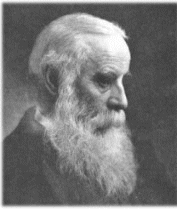
\includegraphics[scale=1]{../graphics/wilson.jpg}
	\caption{John Cook Wilson}
	\label{fig:wilson}
\end{figure}

\section{Description}\label{sec:description} % (fold)

This seminar will concern Oxford reflection on perception in the first half of the twentieth century. Special emphasis will be on how Oxford realism interacts with alien (Cantibrigian and Viennese) influences on theorizing about perception.

Thursday 3-5pm UCL Seminar Room

% section description (end)

\section{Reading}\label{sec:reading} % (fold)

All reading is available at:

\noindent \url{http://markelikalderon.com/teaching/oxford-philosophy-of-perception/}.


\noindent The main reading will be:
\begin{itemize}
	\item G.F. Stout ``Primary and Secondary Qualities''; John Cook Wilson ``Letter to Stout on Primary and Secondary Qualities''
	\item H.A. Prichard chapter 4, ``Phenomena and Things in Themselves'' of \emph{Kant's Theory of Knowledge}
	\item H.A. Prichard ``The Sense Datum Fallacy''
	\item Gilbert Ryle chapter 7, ``Observation and Sensation'', of \emph{The Concept of Mind}
	\item G.A. Paul ``Is There a Problem about Sense Data''
	\item A.J. Ayer chapter 1, ``The Argument from Illusion'' \& chapter 2, ``The Characterization of Sense Data'' of \emph{The Foundations of Empirical Knowledge}
	\item J.L. Austin lectures 9 \& 10 of \emph{Sense and Sensibilia}
	\item H.P. Grice ``The Causal Theory of Perception''
\end{itemize}

\noindent Optional background reading:
\begin{itemize}
	\item M.G.F. Martin ``Sensible Appearances''
	\item M.G.F. Martin ``Austin's \emph{Sense and Sensibilia} revisited''
	\item Mathieu Marion ``Oxford Realism: Knowledge and Perception'' parts \textsc{i} \& \textsc{ii}
	\item Charles Travis ``A Sense of Occasion''
\end{itemize}

% section reading (end)

\end{document}
